\documentclass[a4paper,11pt]{article}

\usepackage[english]{babel}
\usepackage[utf8]{inputenc}
\usepackage[vmargin=3.5cm,hmargin=2cm]{geometry}
\usepackage{graphicx}
\usepackage{amsmath}
\usepackage{mathtools}
\usepackage{fancyhdr}

\setlength{\footskip}{0cm}
\setlength\parindent{0pt} %Quita la sangría francesa
\addtolength{\footskip}{0.8cm}
\addtolength{\headsep}{-.5cm}

\title{\bfseries Report:\\}
\date{}

\lfoot{}
\cfoot{}
\rfoot{\textbf{Signal Theory} \\ Teresa Algarra Ulierte }

\renewcommand{\headrulewidth}{0.5pt}
\renewcommand{\footrulewidth}{0.5pt}

\begin{document}
\renewcommand\contentsname{\vspace{-1cm}}
\maketitle

\begin{centering}
    Teresa Algarra Ulierte \\
    Student ID: teral436 \\
    Personnummer: 970628T129 \\
\end{centering}

\vspace{1cm}

\begin{figure}[!ht]
	\centering
	
\includegraphics[scale = 0.5]{images/portada.jpeg}
\end{figure}

\newpage

\section{Study 1: Modelling Signals}

\subsection{Theoretical Background:}

In this study we will work with white noise, which is defined as a process with constant PSD.

\begin{equation}R_0 = \frac{N_0}{2}\end{equation} 

It is also known that the white noise is Gaussian, which means that if it is WSS, it will be SSS. As we want it to be scalled, we will use $R_x=1$.

We will get this noise through some LTI filters, having:

\begin{equation}R_y(f) = \frac{N_0}{2}|H(f)|^2\end{equation} 

We have a low-degree low-pass filter and an ideal filter:

\begin{figure}[!hp]
    \begin{center}
    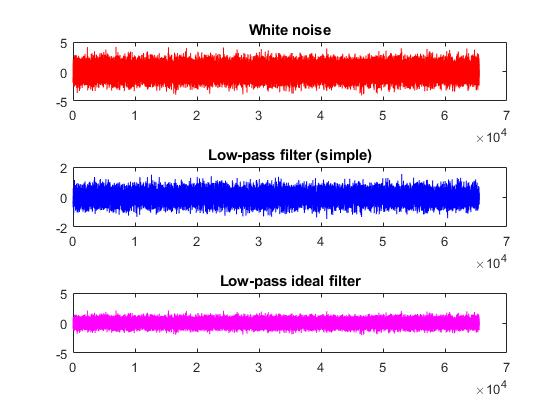
\includegraphics[width=0.6\textwidth]{images/ruidos.jpg}
    \end{center}
\end{figure}

\subsection{Theoretical Analysis:}

To get to calculate the ACF and the PSD of the result function, we have to know exactly what filters we are using. For the low-degree low-pass filter, we will use a first-order Butterworth filter:

\begin{equation}H(z) = \frac{b}{a_1-a_2e^{-j2 \pi f}}\end{equation}

We will use $b = a_1 = 1$ and $a_2 = 0.9$.

For the ideal filter, we can use the rectangle function:

\begin{equation}H[\theta] = rect(\frac{\theta}{\theta_0})\end{equation}

So, we can start by calculating the theoretical PSD knowing the super-formula:

\begin{equation}R_y[\theta] = R_x|H(\theta)|^2\end{equation} 

\newpage

As we are working with White Gaussian Noise, its PSD it's going to be $\frac{N_0}{2}$ as said before, therefore we have:

\begin{equation}R_y[\theta] = \frac{N_0}{2}|H(\theta)|^2\end{equation} 

For the low-degree filter, the result is:

\begin{equation}R_y[\theta] = \frac{N_0}{2}|\frac{b}{a_1-a_2e^{-j2 \pi f}}|^2 = \frac{N_0}{2|1-0.9e^{-j2 \pi f}|^2} \end{equation} 

For the ideal filter, the result is:

\begin{equation}R_y[\theta] = \frac{N_0}{2}|rect(\frac{\theta}{\theta_0})|^2 = \frac{N_0}{2}rect(\frac{\theta}{\theta_0}) = \frac{N_0}{2} if \theta < \theta_0 \end{equation} 

Let's get on to the graphs.

\newpage

\subsubsection{Low-degree filter:}

We get the following PSD when we get the noise through the low-degree low-pass filter:

\begin{figure}[!hp]
    \begin{center}
    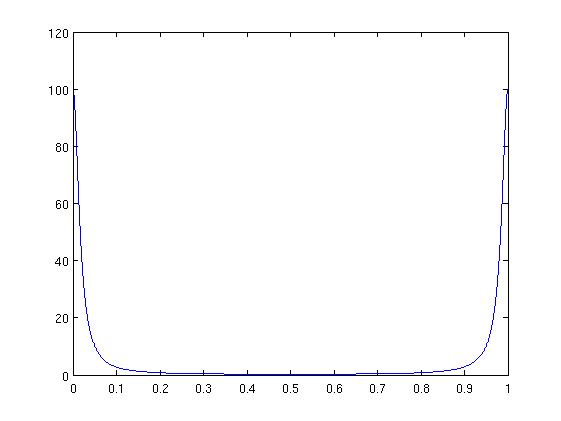
\includegraphics[width=0.6\textwidth]{images/lab1_redo_figure3.jpg}
    \end{center}
\end{figure}

Doing the inverse Fourier transform of the PSD, we get the theoretical ACF, which is:

\begin{figure}[!hp]
    \begin{center}
    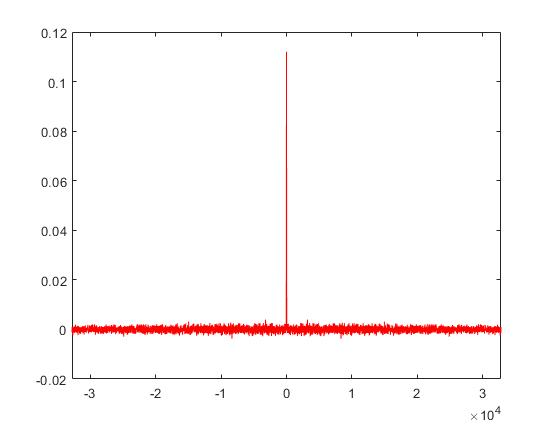
\includegraphics[width=0.6\textwidth]{images/lab2_figure20.jpg}
    \end{center}
\end{figure}

\newpage

\begin{figure}[!hp]
    \begin{center}
    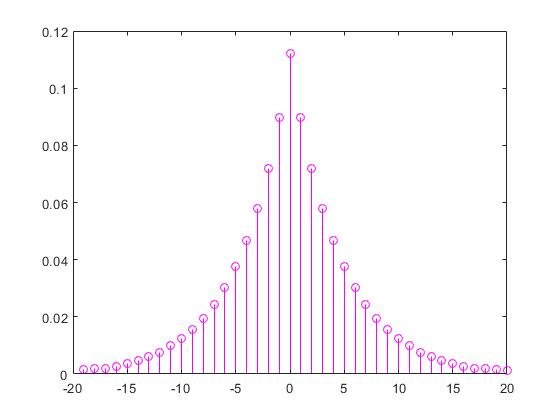
\includegraphics[width=0.6\textwidth]{images/lab2_figure4.jpg}
    \end{center}
\end{figure}

\newpage

\subsubsection{Ideal filter:}

We get the following PSD:

\begin{figure}[!hp]
    \begin{center}
    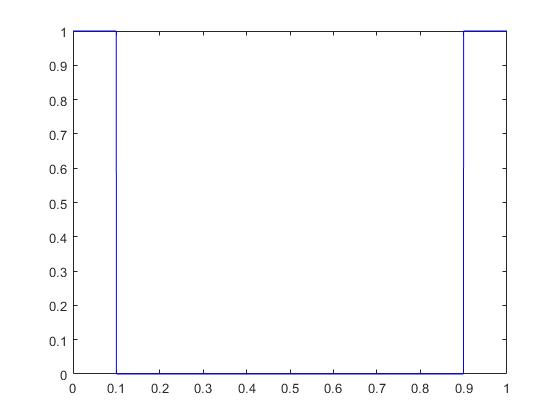
\includegraphics[width=0.6\textwidth]{images/lab3_figure9_1.jpg}
    \end{center}
\end{figure}

With the same calculations as before, we get the ACF:

\begin{figure}[!hp]
    \begin{center}
    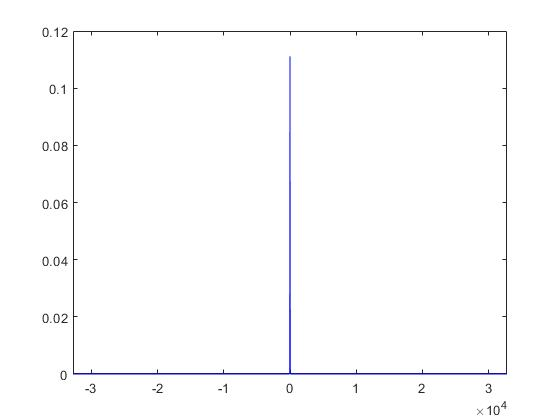
\includegraphics[width=0.6\textwidth]{images/lab2_figure1.jpg}
    \end{center}
\end{figure}

\newpage

\begin{figure}[!hp]
    \begin{center}
    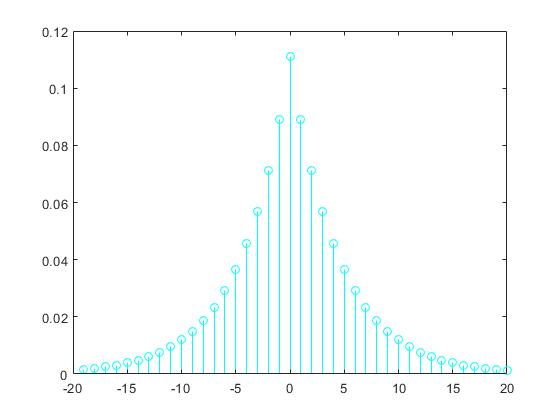
\includegraphics[width=0.6\textwidth]{images/lab2_figure2.jpg}
    \end{center}
\end{figure}

\newpage

\subsection{Estimations:}

\subsubsection{Low-degree filter:}

We will start with the low-degree filter. We will use a first order Butterworth filter. The estimated PSD that we get comes from multiplying the squared absolute value of the filter by the PSD of the input signal, so we get:

\begin{figure}[!hp]
    \begin{center}
    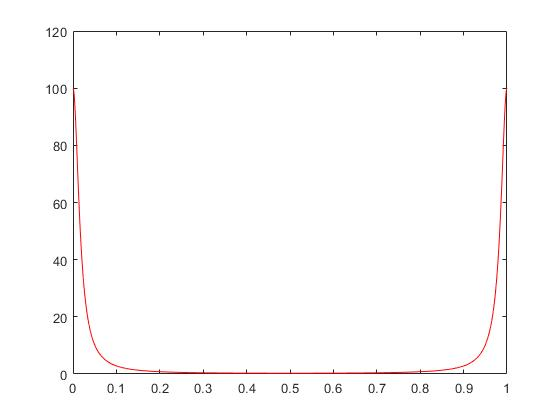
\includegraphics[width=0.6\textwidth]{images/lab1_figure1_3.jpg}
    \end{center}
\end{figure}

Then, for the ACF we use Bartlett's estimation, a funcion that I've defined in a separate script. The result is:

\begin{figure}[!hp]
    \begin{center}
    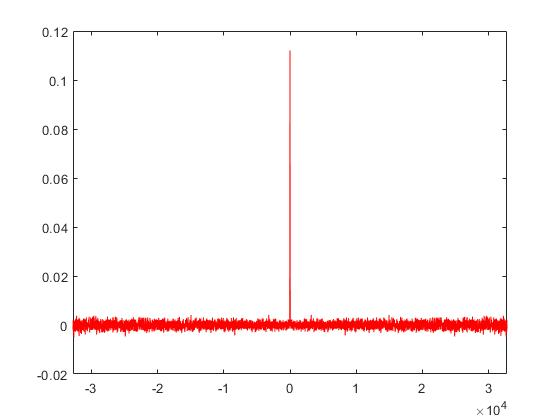
\includegraphics[width=0.6\textwidth]{images/lab2_figure3.jpg}
    \end{center}
\end{figure}

\newpage

\begin{figure}[!hp]
    \begin{center}
    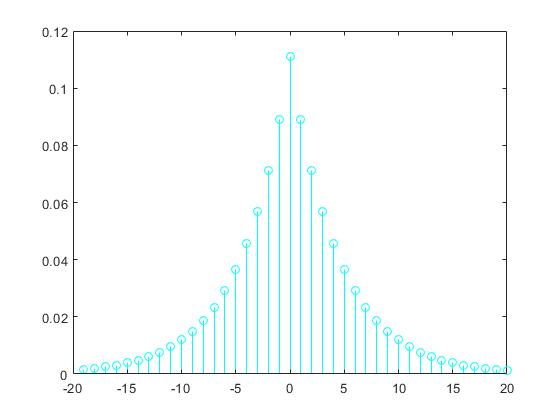
\includegraphics[width=0.6\textwidth]{images/lab2_figure2.jpg}
    \end{center}
\end{figure}

\newpage

\subsubsection{Ideal filter:}

For the ideal filter, the process is exactly the same, but using a tenth order butterworth filter. We get the following PSD, which closed up shows that it's a bit more abrupt that the one from the low-degree filter. It goes symmetric from 0.5 until 1 as the other one.

\begin{figure}[!hp]
    \begin{center}
    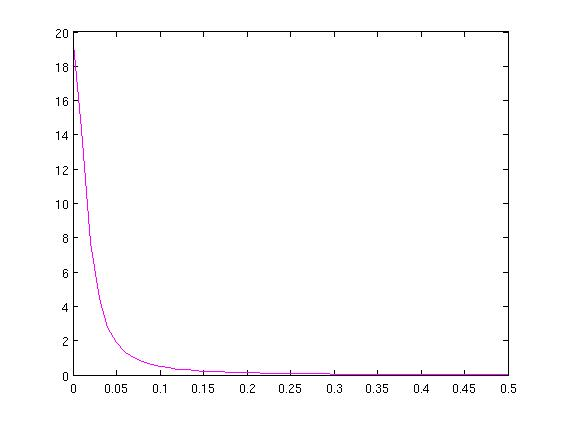
\includegraphics[width=0.6\textwidth]{images/lab1_redo_figure13.jpg}
    \end{center}
\end{figure}

We get the following ACF:

\begin{figure}[!hp]
    \begin{center}
    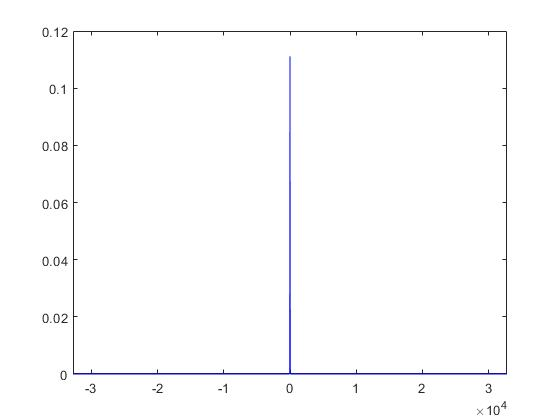
\includegraphics[width=0.6\textwidth]{images/lab2_figure1.jpg}
    \end{center}
\end{figure}

\newpage

\begin{figure}[!hp]
    \begin{center}
    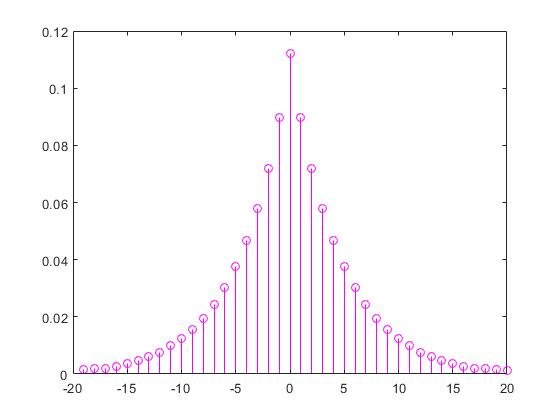
\includegraphics[width=0.6\textwidth]{images/lab2_figure4.jpg}
    \end{center}
\end{figure}

\newpage

\subsection{Final Comparation:}

\begin{itemize}

\item Low-degree filter:

\begin{enumerate}

\item For the low-degree low-pass filter we can see that, regarding the PSD, the estimation does not differ much from the theoretical calculation, as it is almost the same plot.
\item For the ACF, it's also accurate, since the low-degree filter is already not very precise, so the estimations work well.

\end{enumerate}

\item Ideal filter:

\begin{enumerate}

\item For the ideal filter, things definitely differ, as the PSD is a much more smoother curve than the abrupt step that we get in the theoretical calculation.
\item The ACF is much more irregular, our estimation does not give us the steady, straight line that we get in our calculations.

\end{enumerate}

\end{itemize}

\newpage

\section{Study 2:}

\subsection{Theoretical Background:}

In this second study, the aim is to improve the estimates done in the first study. We will use the same White Gaussian noise and both filters. In order to improve our estimations, we have several ways of doing it. We can use \textit{windows}, in which case we have a few possibilities, of which we will explore three of them, \textit{rectangular window}, \textit{Blackman-Harris window} and a \textit{triangle window}.

Here we show the Blackman-Harris window:

\begin{figure}[!hp]
    \begin{center}
    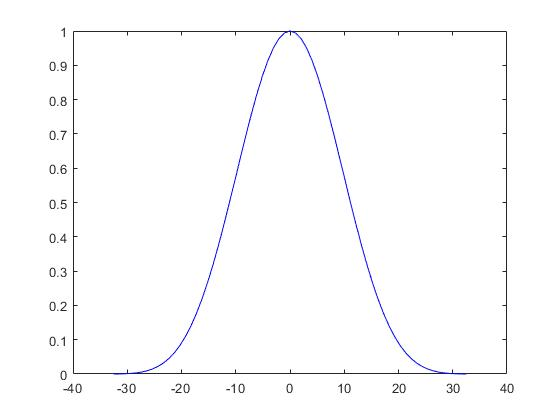
\includegraphics[width=0.6\textwidth]{images/lab2_figure11.jpg}
    \end{center}
\end{figure}

And the triangle window:

\begin{figure}[!hp]
    \begin{center}
    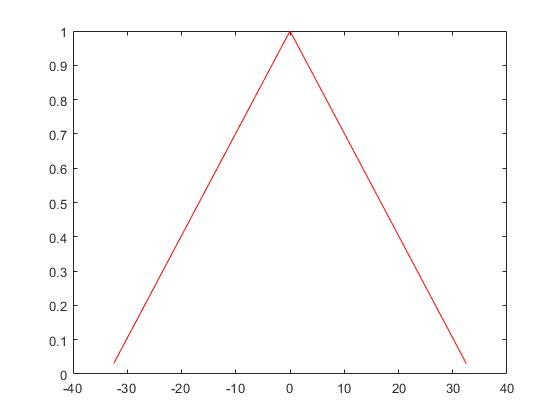
\includegraphics[width=0.6\textwidth]{images/lab2_figure13.jpg}
    \end{center}
\end{figure}

\subsection{Improved Estimations:}

\subsubsection{Ideal filter:}

We will start exploring the ACF of the ideal filter. Using the previously defined functions, we get this plots:

\begin{figure}[!hp]
    \begin{center}
    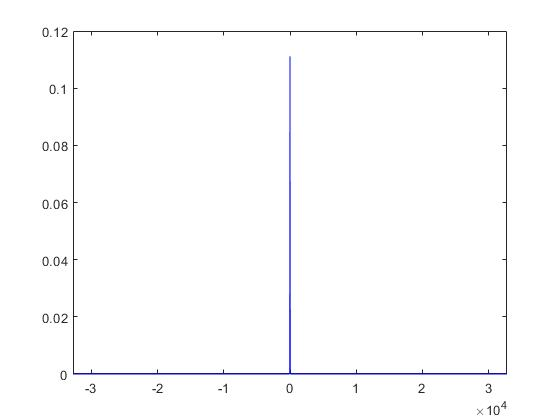
\includegraphics[width=0.6\textwidth]{images/lab2_figure1.jpg}
    \end{center}
\end{figure}

\begin{figure}[!hp]
    \begin{center}
    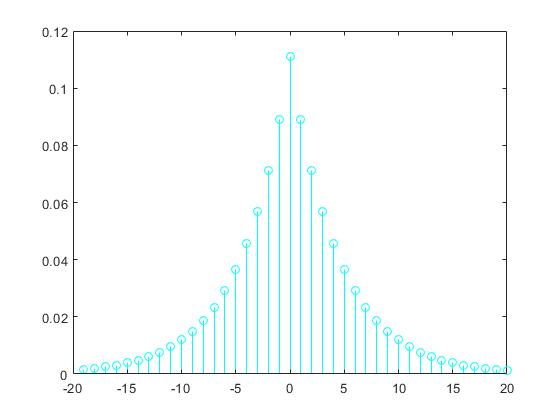
\includegraphics[width=0.6\textwidth]{images/lab2_figure2.jpg}
    \end{center}
\end{figure}

\newpage

We can also estimate the ACF with the Bartlett method, having these results:

\begin{figure}[!hp]
    \begin{center}
    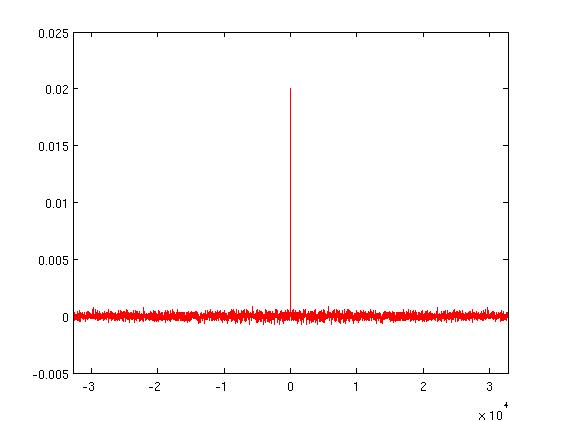
\includegraphics[width=0.6\textwidth]{images/lab2_redo_figure13.jpg}
    \end{center}
\end{figure}

\begin{figure}[!hp]
    \begin{center}
    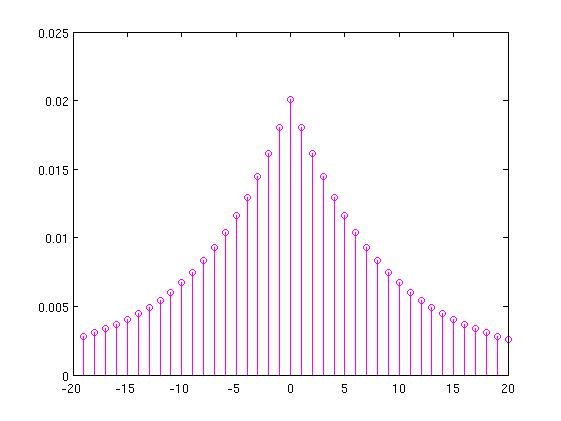
\includegraphics[width=0.6\textwidth]{images/lab2_redo_figure14.jpg}
    \end{center}
\end{figure}

\newpage

We now get on to the theoretical PSD we get from the filtered signal:

\begin{figure}[!hp]
    \begin{center}
    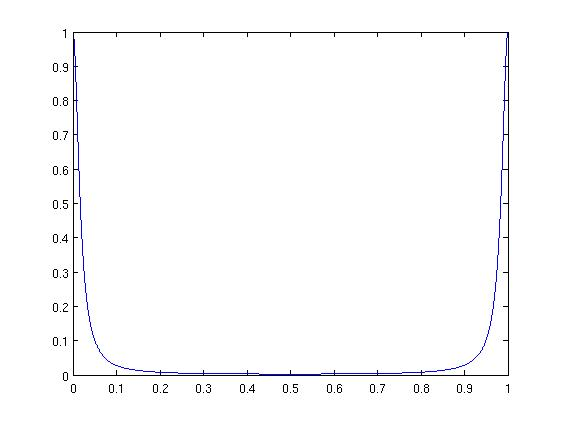
\includegraphics[width=0.6\textwidth]{images/lab2_redo_figure2.jpg}
    \end{center}
\end{figure}

Moving on to the estimations, here we have the original estimated periodogram for our signal.

\begin{figure}[!hp]
    \begin{center}
    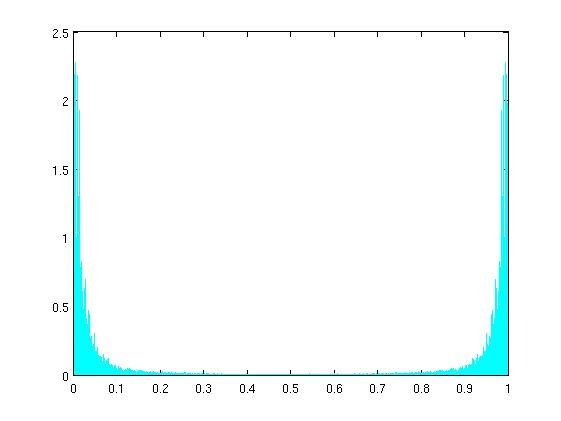
\includegraphics[width=0.6\textwidth]{images/lab2_redo_figure3.jpg}
    \end{center}
\end{figure}

\newpage

Now we calculate the averaged periodogram:

\begin{figure}[!hp]
    \begin{center}
    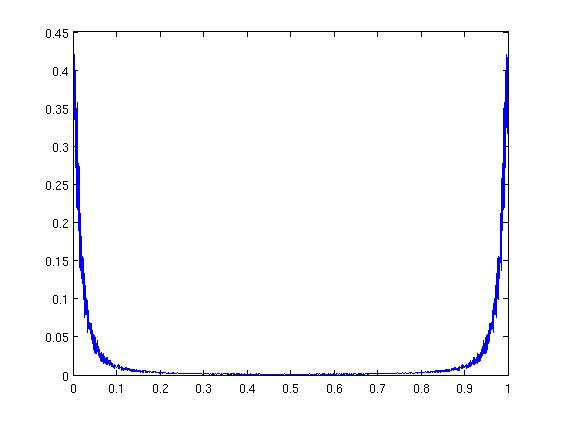
\includegraphics[width=0.6\textwidth]{images/lab2_redo_figure4.jpg}
    \end{center}
\end{figure}

And finally we move on to our improved estimations. Here we have the smoothed periodogram with the rectangular window:

\begin{figure}[!hp]
    \begin{center}
    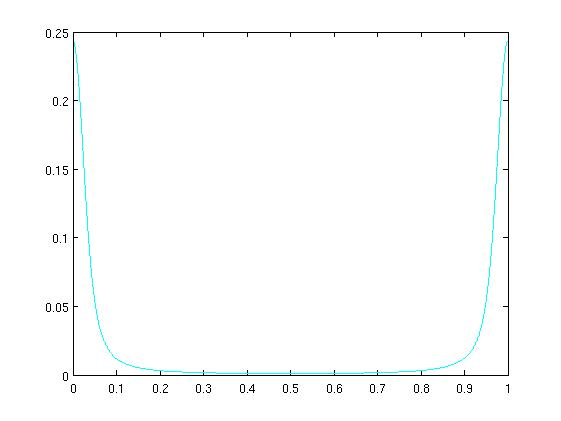
\includegraphics[width=0.6\textwidth]{images/lab2_redo_figure5.jpg}
    \end{center}
\end{figure}

\newpage

This is the periodrogram gotten through the Blackman-Harris window:

\begin{figure}[!hp]
    \begin{center}
    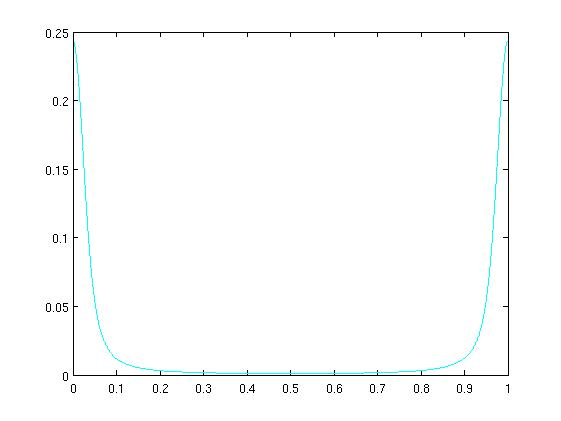
\includegraphics[width=0.6\textwidth]{images/lab2_redo_figure6.jpg}
    \end{center}
\end{figure}

And this is the one we get through the triangle window:

\begin{figure}[!hp]
    \begin{center}
    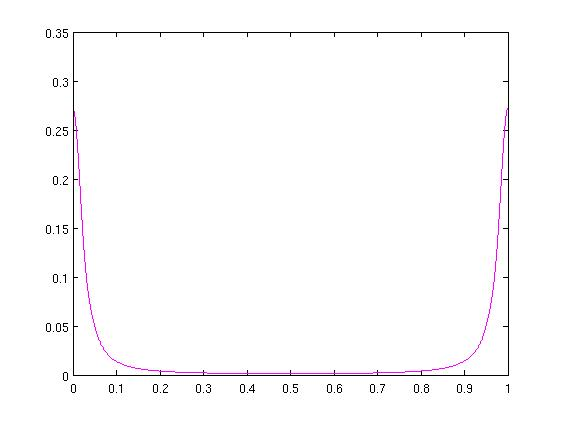
\includegraphics[width=0.6\textwidth]{images/lab2_redo_figure7.jpg}
    \end{center}
\end{figure}

\newpage

\subsubsection{Low-degree filter:}

Let's move on to the low-degree filter, starting with the ACF:

\begin{figure}[!hp]
    \begin{center}
    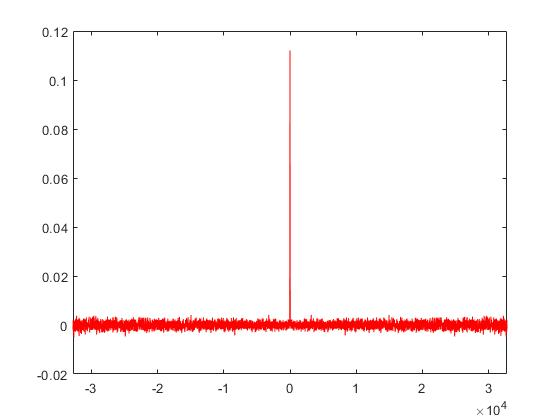
\includegraphics[width=0.6\textwidth]{images/lab2_figure3.jpg}
    \end{center}
\end{figure}

\begin{figure}[!hp]
    \begin{center}
    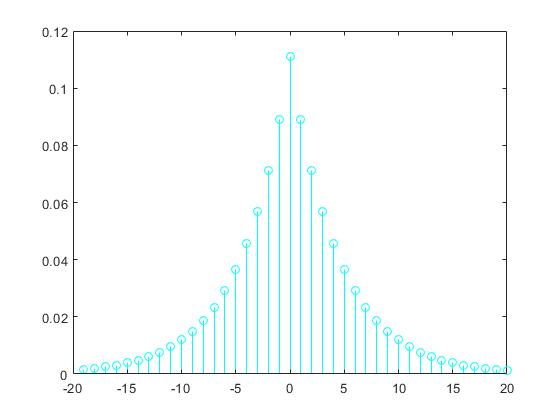
\includegraphics[width=0.6\textwidth]{images/lab2_figure2.jpg}
    \end{center}
\end{figure}

\newpage

We can also estimate the ACF with the Bartlett method, having these results:

\begin{figure}[!hp]
    \begin{center}
    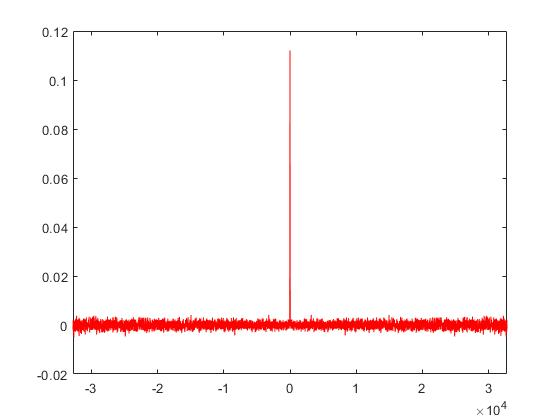
\includegraphics[width=0.6\textwidth]{images/lab2_figure3.jpg}
    \end{center}
\end{figure}

\begin{figure}[!hp]
    \begin{center}
    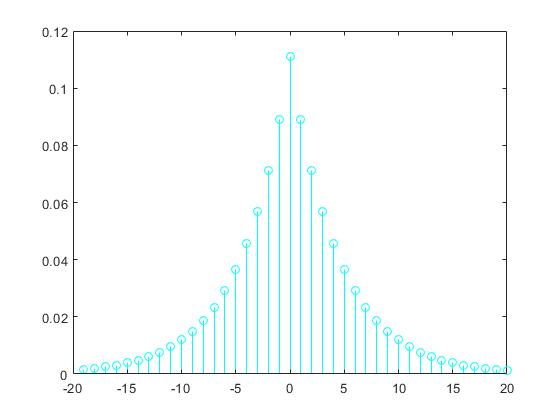
\includegraphics[width=0.6\textwidth]{images/lab2_figure2.jpg}
    \end{center}
\end{figure}

\newpage

We now get on to the theoretical PSD we get from the filtered signal:

\begin{figure}[!hp]
    \begin{center}
    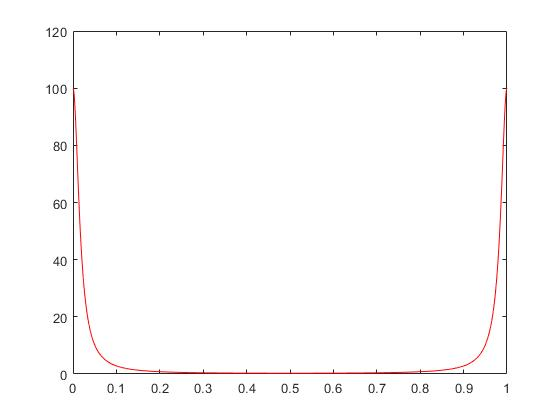
\includegraphics[width=0.6\textwidth]{images/lab1_figure1_3.jpg}
    \end{center}
\end{figure}

Going to the estimations, here we have the original estimated periodogram for our signal.

\begin{figure}[!hp]
    \begin{center}
    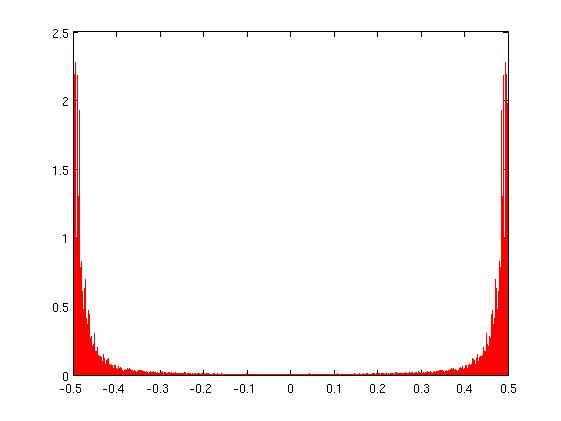
\includegraphics[width=0.6\textwidth]{images/lab2_redo_figure15.jpg}
    \end{center}
\end{figure}

\newpage

Now we calculate the averaged periodogram:

\begin{figure}[!hp]
    \begin{center}
    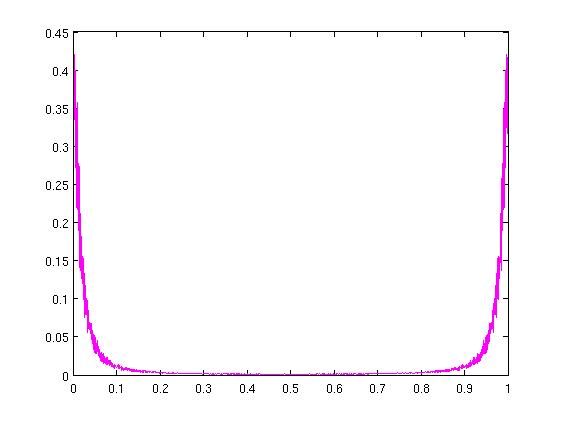
\includegraphics[width=0.6\textwidth]{images/lab2_redo_figure16.jpg}
    \end{center}
\end{figure}

And finally, the improved estimations. Here we have the periodogram taken through the rectangular window:

\begin{figure}[!hp]
    \begin{center}
    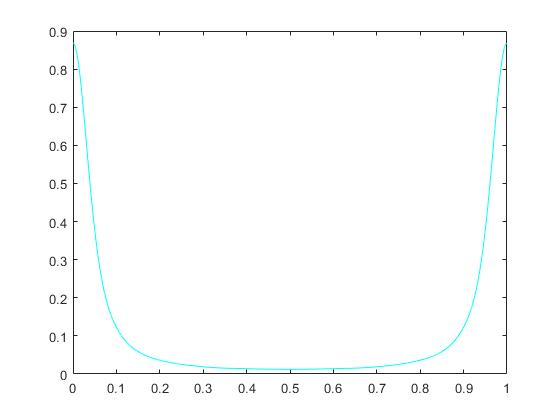
\includegraphics[width=0.6\textwidth]{images/lab2_figure10.jpg}
    \end{center}
\end{figure}

\newpage

This is the periodrogram gotten through the Blackman-Harris window:

\begin{figure}[!hp]
    \begin{center}
    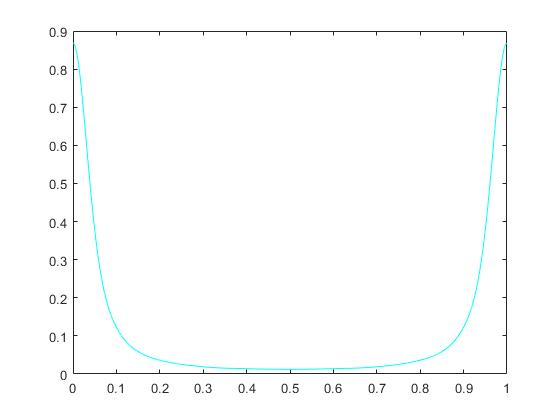
\includegraphics[width=0.6\textwidth]{images/lab2_figure12.jpg}
    \end{center}
\end{figure}

And this is the one we get through the triangle window:

\begin{figure}[!hp]
    \begin{center}
    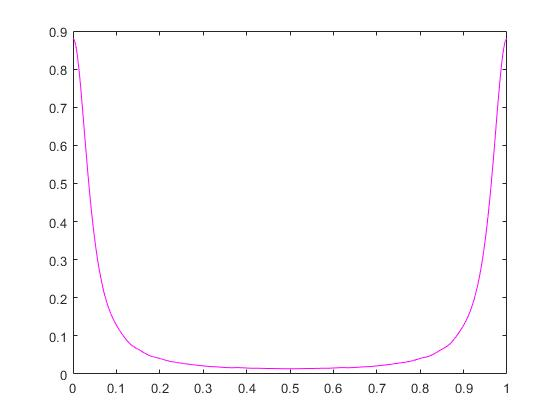
\includegraphics[width=0.6\textwidth]{images/lab2_figure14.jpg}
    \end{center}
\end{figure}

\newpage

\subsection{Final Conclusion:}

As we can see, the ones we estimate are much more smoothier and have an unique line or curve, in stead of being a messy signal with ups and downs as are they raw and averaged periodograms. The look much more like the theoretical PSD we get, meaning they have a cleaner and closer approach to the calculations we have done before-hand. Still, they're much smoother and less abrupt than the estimations for the ideal filter, since, after all, they are still estimations.

\newpage

\section{Study 3:}

\subsection{Theoretical Background:}

We have the three following systems:

A squarer:

\begin{equation}
  Y[n] =X^2[n]
\end{equation}

A half-wave rectifier:

\begin{equation}
  Y[n] =
    \begin{cases}
        X[n],& n: X[n]>0,\\
        0,    & n: X[n] \leq 0,
    \end{cases}
\end{equation}

An AM-SC modulator:

\begin{equation}
  Y[n] =X[n]cos(\Omega_{0} n)
\end{equation}

As we can see, non of them is LTI, which means that the output might or might not be Gaussian, and which also means that the PSD does not follow the formula we normally use, but an specific formula for the kind of non-linearity that the system presents. 

Therefore, we have three special formulas:

\begin{equation}
  r_Y(\tau) = 2r_X^2(\tau) + r_X^2(0)
\end{equation}

\begin{equation}
  r_Y(\tau) = \frac{r_X(0)}{2\pi} + \frac{r_X(\tau)}{4} + \frac{r_X^2(\tau)}{4\pi r_X(o)} + ...
\end{equation}

\begin{equation}
  r_Y(\tau) = \frac{A^2}{2}(C^2 + r_X(\tau))cos(2\pi f_c \tau)
\end{equation}

They belong respectively with each one of the transformations above.

Knowing the value of $R_x(\tau)$, and therefore the value of $r_x(\tau)$, we translate them to the frequency domain to have the PSD expressions:

\begin{equation}
  R_Y[\theta] = 4\theta_c\Lambda[\frac{\theta}{2\theta_c}]+4\theta_c^2\delta[\theta]
\end{equation}

\begin{equation}
 R_Y[\theta] = \frac{1}{4\pi}\Lambda[\frac{\theta}{2\theta_c}]+\frac{1}{4}rect[\frac{\theta} {2\theta_c}]
+\frac{\theta_c}{\pi}\delta[\theta]
\end{equation}

\begin{equation}
  R_Y[\theta] = \frac{1}{4}(rect[\frac{\theta+\Omega_{0}} {2\theta_c}]+rect[\frac{\theta-\Omega_{0}} {2\theta_c}])
\end{equation}

\newpage

As done in the previous studies, we will use input noise:

\begin{figure}[!hp]
    \begin{center}
    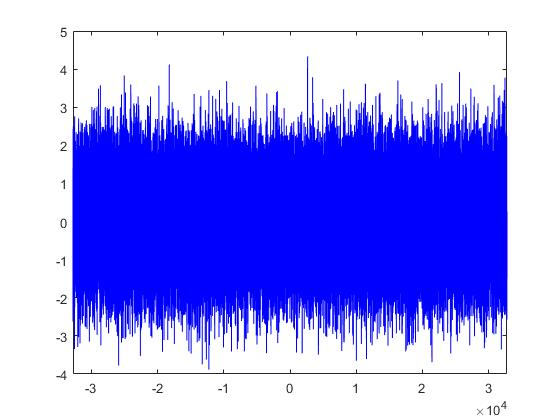
\includegraphics[width=0.6\textwidth]{images/lab3_figure1_1.jpg}
    \end{center}
\end{figure}

We will get it through in ideal low-pass filter, having the following result:

\begin{figure}[!hp]
    \begin{center}
    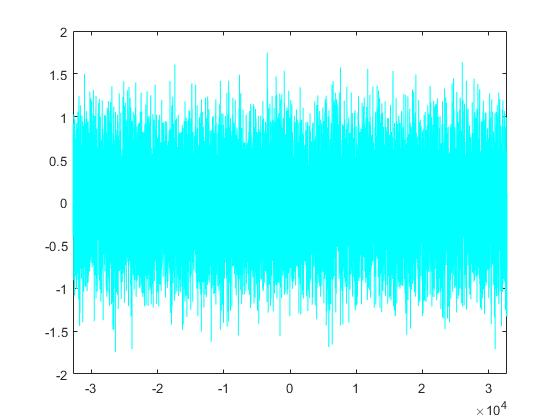
\includegraphics[width=0.6\textwidth]{images/lab3_figure1_2.jpg}
    \end{center}
\end{figure}

\newpage

The systems have the following representation:

This is the squarer system:

\begin{figure}[!hp]
    \begin{center}
    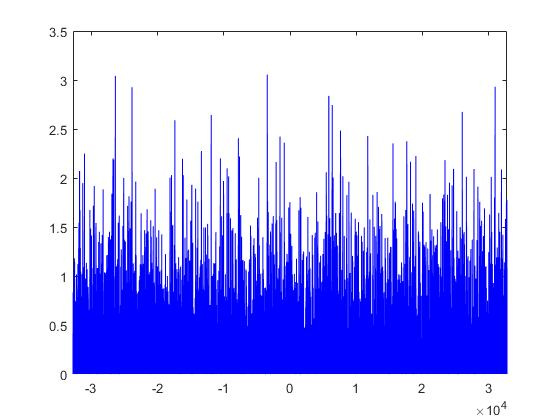
\includegraphics[width=0.6\textwidth]{images/lab3_figure2_1.jpg}
    \end{center}
\end{figure}

This is the half-wave rectifier:

\begin{figure}[!hp]
    \begin{center}
    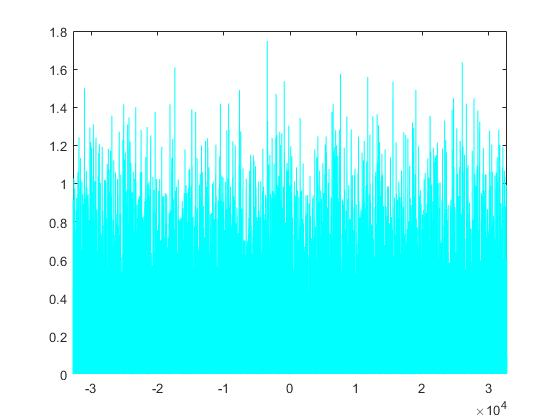
\includegraphics[width=0.6\textwidth]{images/lab3_figure2_2.jpg}
    \end{center}
\end{figure}

\newpage

This is the AM-SC modulator:

\begin{figure}[!hp]
    \begin{center}
    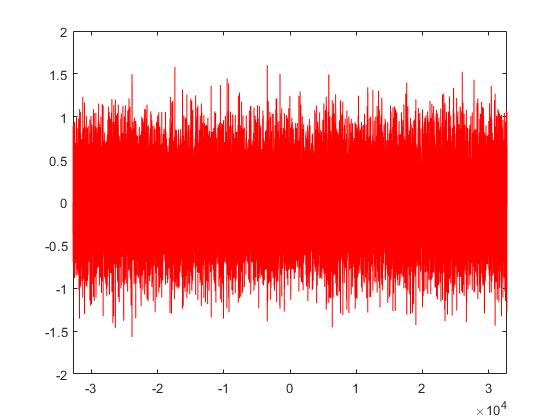
\includegraphics[width=0.6\textwidth]{images/lab3_figure2_3.jpg}
    \end{center}
\end{figure}

As it is obvious from the equations, the two first systems are only positive, whereas the third one isn't necessarily positive, it can have negative values.

\newpage

\subsection{Theoretical Analysis:}

First we can start with the PSD. We use the funtions that we have already used in previous studies, resulting in a PSD for the filter signal with the following plot:

\begin{figure}[!hp]
    \begin{center}
    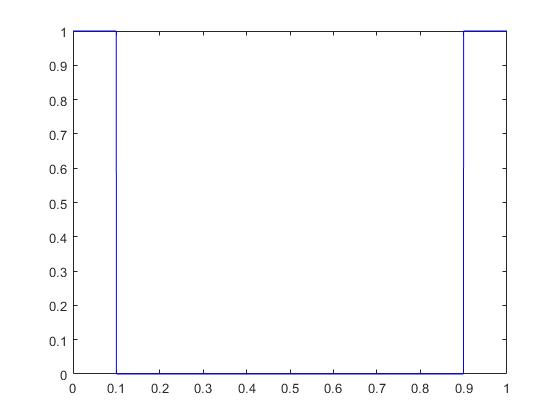
\includegraphics[width=0.6\textwidth]{images/lab3_figure9_1.jpg}
    \end{center}
\end{figure}

If we get the signal through the squarer, the resulting PSD is:

\begin{figure}[!hp]
    \begin{center}
    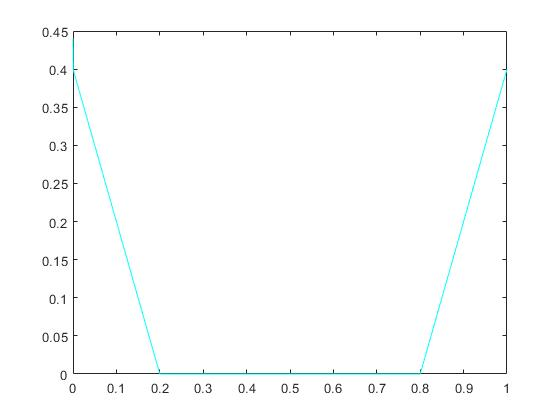
\includegraphics[width=0.6\textwidth]{images/lab3_figure9_2.jpg}
    \end{center}
\end{figure}

\newpage

The PSD that we get after applying the half-wave rectifier to the filtered signal is:

\begin{figure}[!hp]
    \begin{center}
    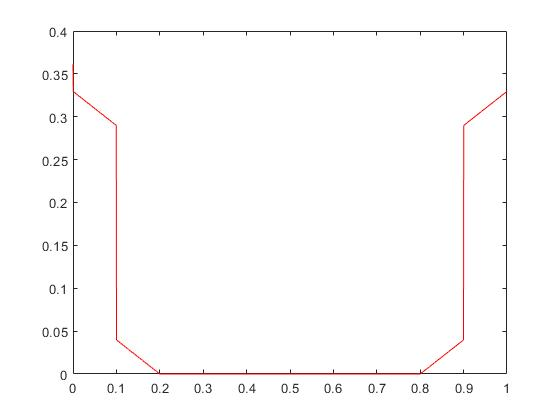
\includegraphics[width=0.6\textwidth]{images/lab3_figure9_3.jpg}
    \end{center}
\end{figure}

Lastly, the PSD resulting from AM-SC modulating the signal is:

\begin{figure}[!hp]
    \begin{center}
    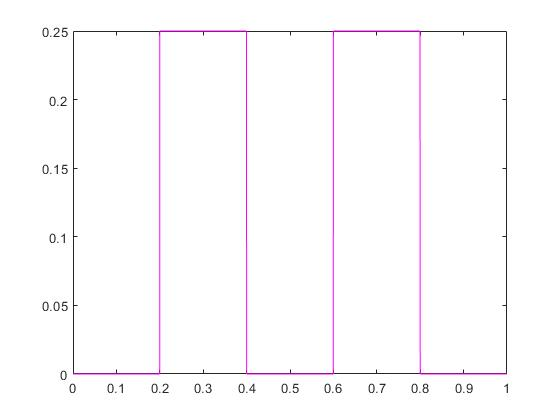
\includegraphics[width=0.6\textwidth]{images/lab3_figure9_4.jpg}
    \end{center}
\end{figure}

\newpage

\subsection{Periodograms and historiograms:}

We can continue with the periodograms of the three non-linear systems.

For the squarer, the plot resulting of applying our defined Periodogram function is:

\begin{figure}[!hp]
    \begin{center}
    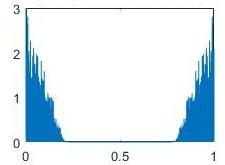
\includegraphics[width=0.6\textwidth]{images/lab3_figure10.jpg}
    \end{center}
\end{figure}

Then we have the following plot for the half-wave rectifier:

\begin{figure}[!hp]
    \begin{center}
    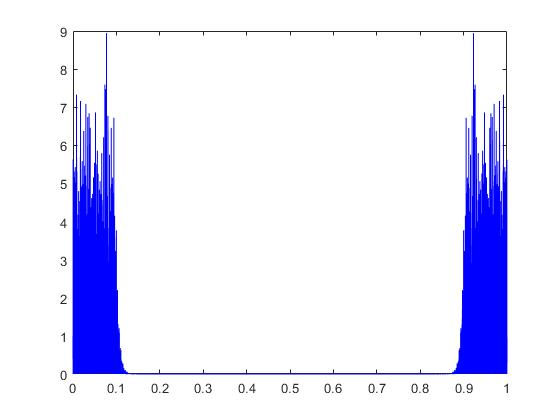
\includegraphics[width=0.6\textwidth]{images/lab3_figure10_1.jpg}
    \end{center}
\end{figure}

\newpage

Then, we get this periodogram for the AM-SC modulator:

\begin{figure}[!hp]
    \begin{center}
    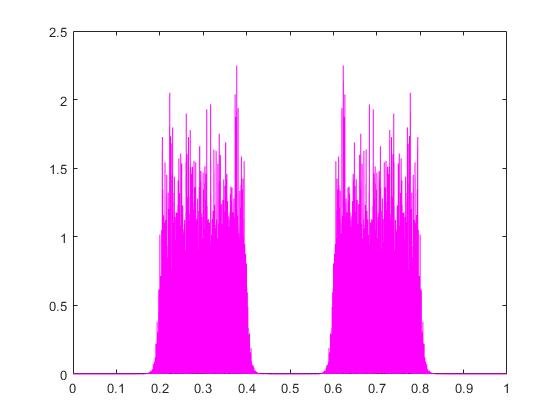
\includegraphics[width=0.6\textwidth]{images/lab3_figure10_4.jpg}
    \end{center}
\end{figure}

The last thing we will calculate in this section is the historiogram of each one of our systems.

First, the historiogram of our signal Y:

\begin{figure}[!hp]
    \begin{center}
    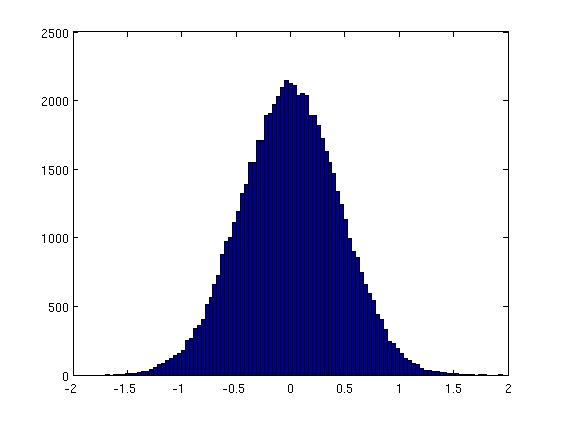
\includegraphics[width=0.6\textwidth]{images/lab3_redo_33.jpg}
    \end{center}
\end{figure}

\newpage

This is the one for the squarer:

\begin{figure}[!hp]
    \begin{center}
    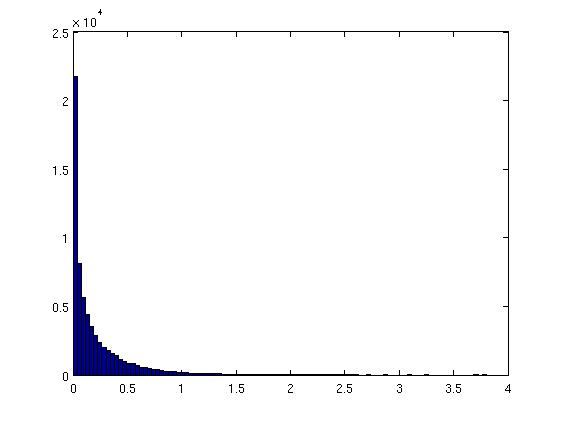
\includegraphics[width=0.6\textwidth]{images/lab3_redo_34.jpg}
    \end{center}
\end{figure}

We have the following historiogram for the half-wave rectifier:

\begin{figure}[!hp]
    \begin{center}
    \includegraphics[width=0.6\textwidth]{images/lab3_redo_35.jpg}
    \end{center}
\end{figure}

\newpage

Finally, this is the plot of the historiogram of the AM-SC modulator:

\begin{figure}[!hp]
    \begin{center}
    \includegraphics[width=0.6\textwidth]{images/lab3_redo_36.jpg}
    \end{center}
\end{figure}

\newpage

\subsection{Estimations:}

We will plot the estimations for the PSD. We will smooth them with a rectangular window. 

If we get the signal through the squarer, the resulting PSD is:

\begin{figure}[!hp]
    \begin{center}
    \includegraphics[width=0.6\textwidth]{images/lab3_redo_26.jpg}
    \end{center}
\end{figure}

The PSD that we get after applying the half-wave rectifier to the filtered signal is:

\begin{figure}[!hp]
    \begin{center}
    \includegraphics[width=0.6\textwidth]{images/lab3_redo_27.jpg}
    \end{center}
\end{figure}

\newpage

Lastly, the PSD resulting from AM-SC modulating the signal is:

\begin{figure}[!hp]
    \begin{center}
    \includegraphics[width=0.6\textwidth]{images/lab3_redo_28.jpg}
    \end{center}
\end{figure}

\subsection{Final Comparation:}

\begin{itemize}

\item We can assume that the theoretical calculations for the PSD as pretty accurate, since the estimated plots are a more curved or smoothed version of the calculated PSD, given that no real process has such an abrupt change in its PSD. 

\item In the periodograms, we can see how differently the signal changes depending on the system. On the AM-SC modulator, we have two peaks in the middle, whereas in the squarer, we have two symmetrical decreasing signals on the corner of the plot, for example. This can give us an idea of how the system will work.

\item Lastly, the historiograms are very different among them. We can see how well distributed is the one from our signal Y, and then how the squarer and the half-wave rectifier make it only positive and way more abrupt. With the AM-SC modulator, we still have the negative part but it becomes, once again, more abrupt, with a remarkable slop.

\end{itemize}

\newpage

\section{Study 4:}

\subsection{Theoretical Background:}

We hace two special operations:

\begin{equation}
  Y[n] = X[n](-1)^n
\end{equation}

\begin{equation}
  Y[n] =
    \begin{cases}
        X[n],& n: odd,\\
        0,    & n: even\\
    \end{cases}
\end{equation}

These represent two ways in which signals can be manipulated. We will get our every-study low-pass filtered White Gaussian Noise through these systems, to see if they're still WSS and to analize what happends with the PSDs of the signals that are being manipulated in this way in our every-day life situations.

We have to calculate the PSD from the ACF:

\begin{equation}
  r_Y[\theta] = E\{Y[n+\theta]Y[n]\}
\end{equation}

I will not describe all the intermediate steps calculated here, so the final PSD result after the Fourier transform is for the first alternating system:

\begin{equation}
  R_Y[\theta] = R_X[\theta-0.5]
\end{equation}

And for the second system:

\begin{equation}
  R_Y[\theta] = \frac{1}{4}(R_X[\theta-0.5] + R_X[\theta])
\end{equation}

\newpage

\subsection{Theoretical Analysis:}

First we will start showing the plots of the theoretical PSD. Here is the PSD of the signal put through the first system:

\begin{figure}[!hp]
    \begin{center}
    \includegraphics[width=0.6\textwidth]{images/lab4_figure11.jpg}
    \end{center}
\end{figure}

And here we have the PSD of the signal after the second system:

\begin{figure}[!hp]
    \begin{center}
    \includegraphics[width=0.6\textwidth]{images/lab4_figure12.jpg}
    \end{center}
\end{figure}

\newpage

\subsection{Estimations:}

Leaving behind the theoretical calculations, we can move one to the estimations done, so we will go to the PSD estimation for the first case:

\begin{figure}[!hp]
    \begin{center}
    \includegraphics[width=0.6\textwidth]{images/lab4_figure7.jpg}
    \end{center}
\end{figure}

This plot is the PSD estimation for the first system:

\begin{figure}[!hp]
    \begin{center}
    \includegraphics[width=0.6\textwidth]{images/lab4_figure8.jpg}
    \end{center}
\end{figure}

\newpage

And this is the PSD associated to the last manipulation described:

\begin{figure}[!hp]
    \begin{center}
    \includegraphics[width=0.6\textwidth]{images/lab4_figure9.jpg}
    \end{center}
\end{figure}

\subsection{Final Comparation:}

As we can see, the estimated PSD is a messy version of the theoretical PSD, so we can assume that, if we filter it and smoothed it, we would have the same PSD. That shows that the calculations are correct, but that the systems are putting a lot of noise in the resulting plots.

\vspace{4cm}

\end{document}
